\chapter{Симуляция базовых эмоций в трёхмерной модели}
\label{chap:results}
В системе, полученной из трёх совмещённых систем нейромодуляторов на языке Python, с общим словарём областей мозга, выделенными для них нейронами в реалистичных пропорциях и настроенными связями, была проведена симуляция на 150 000 нейронов. Симулировалась работа мозга в течение 1400 миллисекунд, за это время нейромодуляторы принимали различные значения, приводящие "мозг" в 8 различных состояний:


1. Эмоция «тоска/горе». Требует высокого уровня норадреналина при низких уровнях дофамина и серотонина. Генераторы спайков подключены к ядрам солитарного тракта, ядрам paragigantocellular, латерально-спинному ядру покрышки и perirphinal cortex с 100 по 200 мс.


2. Эмоция «испуг/ужас». Формируется при высоком уровне дофамина и низких уровнях серотонина и норадреналина. Генераторы спайков подключены к моторной коре, чёрной субстанции pars compacta, миндалевидному телу и вентральной области покрышки с 300 по 400 мс.


3. Эмоция «злость/ярость». Возникает при высоких уровнях норадреналина и  дофамина, а активность одного из них всегда влечёт активность другого. С 500 по 600 мс генерируются спайки на ядрах солитарного тракта, ядрах paragigantocellular, латерально-спинном ядре покрышки и perirphinal cortex. Вместе с ними работают генераторы на моторной коре, чёрной субстанции pars compacta, миндалевидном теле и вентральной области покрышки.


4. Эмоция «презрение/отвращение». Требует высокого уровня серотонина при низких уровнях дофамина и норадреналина. Генераторы спайков с 700 по 800 мс подключены к серотониновым очагам в префронтальной коре, моторной коре и ядрах шва (дорсальном и среднем).


5. Эмоция «удивление». Высокие уровни серотонина и норадреналина, норадреналин борется за сохранение своего возбуждающего влияния, но не в полной мере сохраняет его под ингибирующим действием серотонина. К генераторам в префронтальной коре, моторной коре, дорсальном и среднем ядрах шва добавляются генераторы на ядрах солитарного тракта, ядрам paragigantocellular, латерально-спинному ядру покрышки и perirphinal cortex, вместе они работают с 900 по 1000 мс.


6. Эмоция «радость/удовольствие». Требует одновременного существования спайковой активности в центрах дофамина и серотонина (чтобы серотонин не подавил дофамин), для чего были созданы центры ---------------- в --------. 1100 по 1200 мс. Концентрация норадреналина должна оставаться низкой. 


7. Эмоция «интерес/азарт». Высокие уровни всех трёх нейромедиаторов. Генераторы спайков в центрах дофамина (моторной коре, чёрной субстанции pars compacta, миндалевидном теле и вентральной области покрышки), генераторы в центрах серотонина (префронтальная кора, моторная кора, дорсальное и среднее ядра шва), генераторы активности норадреналина (на ядрах солитарного тракта, ядрах paragigantocellular, латерально-спинном ядре покрышки и perirphinal cortex) включаются одновременно на 1300 мс, работают до 1400 мс.

8. Эмоция «стыд/унижение». Пониженные уровни всех трёх нейромедиаторов в промежутках между остальными выражаемыми эмоциями.

На сервере CISCO симуляция, распределённая на 8 потоков, заняла 17 часов, поскольку была намеренно облегчена нагрузка: детекторы спайков и вольтметры были подключены лишь к наиболее важным для анализа областям мозга. Этими частями стали: \begin{itemize}
\item Нейромодулирующие центры (ядра шва, голубоватое пятно, чёрная субстанция pars compacta);


\begin{figure}
	\centering
	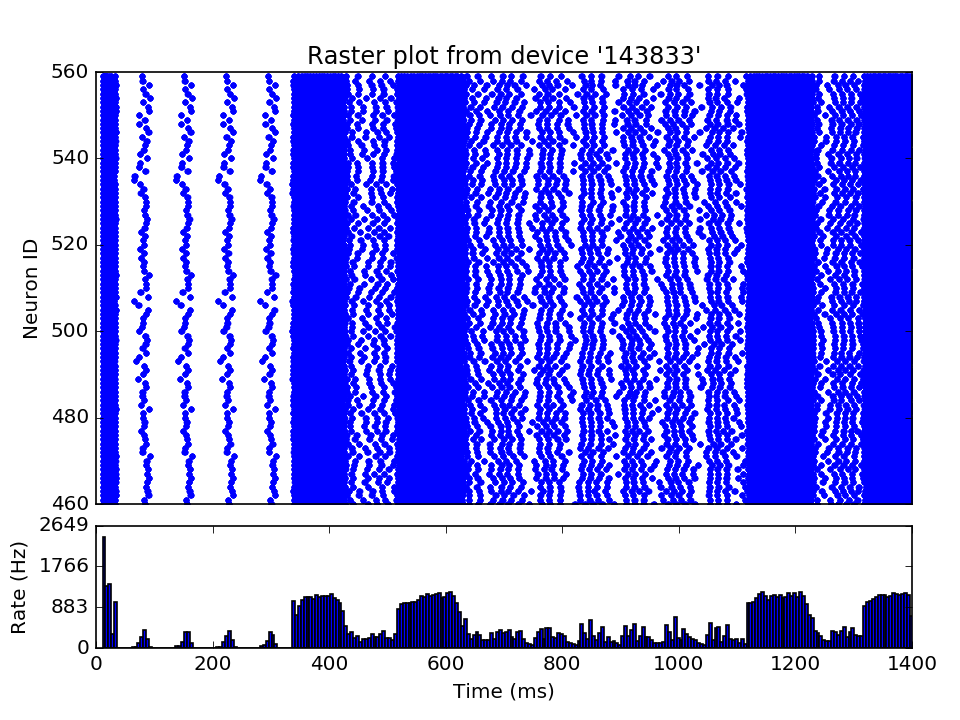
\includegraphics[width=0.5\linewidth]{spikes_lc[d1]}
	\caption{Спайковая активность в голубоватом ядре.}
	\label{fig:spikes_lc[d1]}
\end{figure}

\begin{figure}
	\centering
	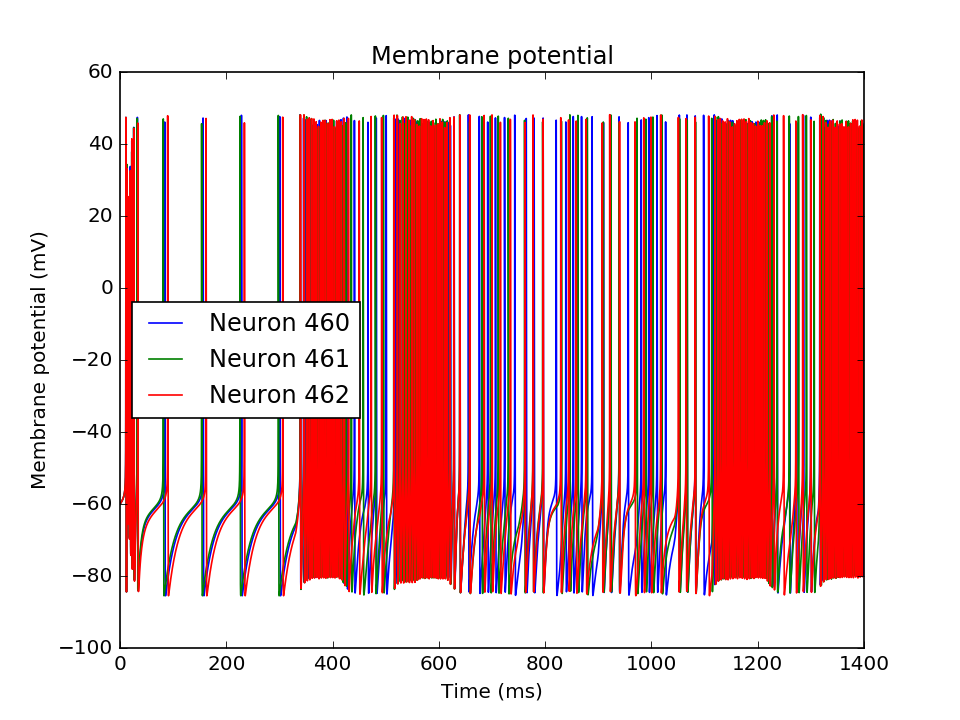
\includegraphics[width=0.5\linewidth]{volt_lc[d1]}
	\caption{Изменение потенциала мембраны нескольких нейронов в голубоватом ядре.}
	\label{fig:volt_lc[d1]}
\end{figure}

\begin{figure}
	\centering
	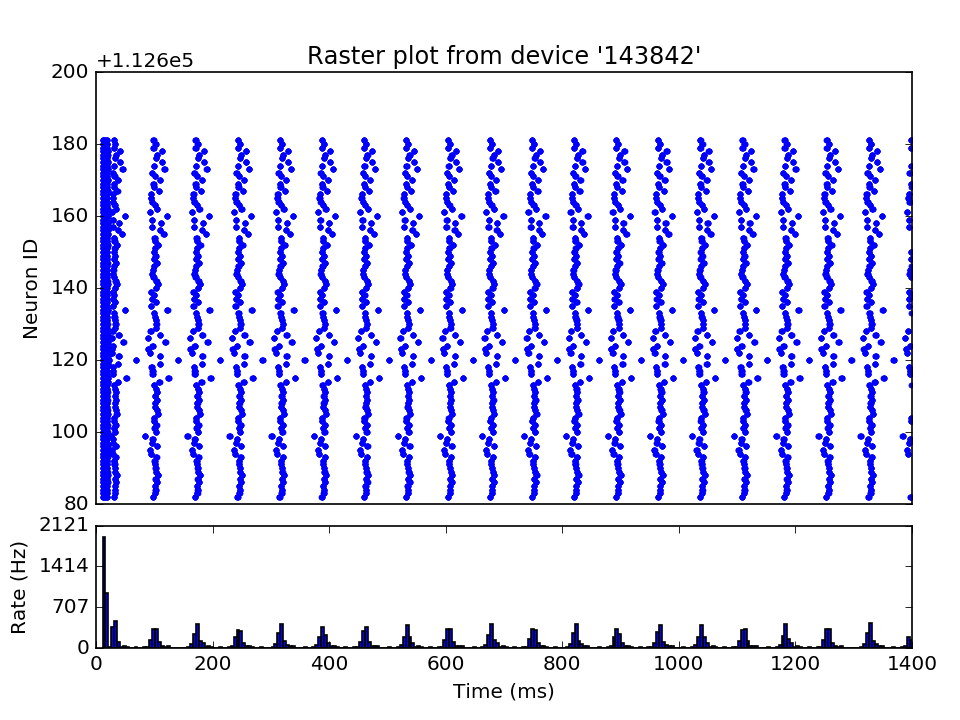
\includegraphics[width=0.5\linewidth]{spikes_rn[a1]}
	\caption{Спайковая активность в ядрах шва.}
	\label{fig:spikes_rn[a1]}
\end{figure}

\begin{figure}
	\centering
	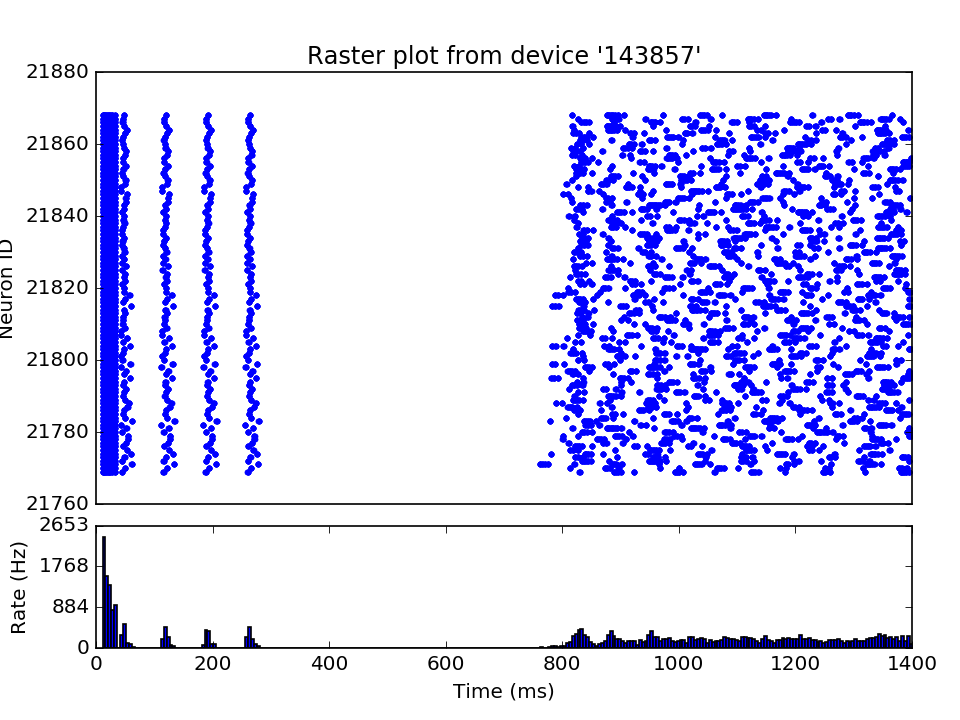
\includegraphics[width=0.5\linewidth]{spikes_snc[gaba]}
	\caption{Спайковая активность в чёрной субстанции pars compacta.}
	\label{fig:sero600voltage}
\end{figure}

\item Интерфейсы нейромодуляторов (стриатум, таламус, вентральная область покрышки);


\begin{figure}
	\centering
	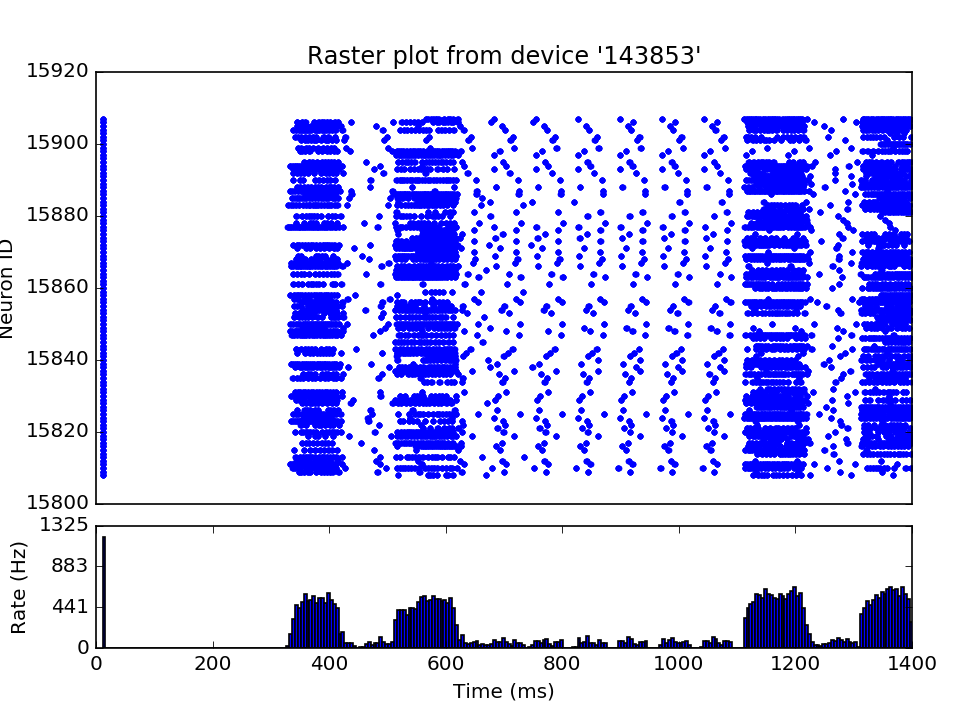
\includegraphics[width=0.5\linewidth]{spikes_vta[da0]}
	\caption{Спайковая активность в вентральной области покрышки.}
	\label{fig:spikes_vta}
\end{figure}

\begin{figure}
	\centering
	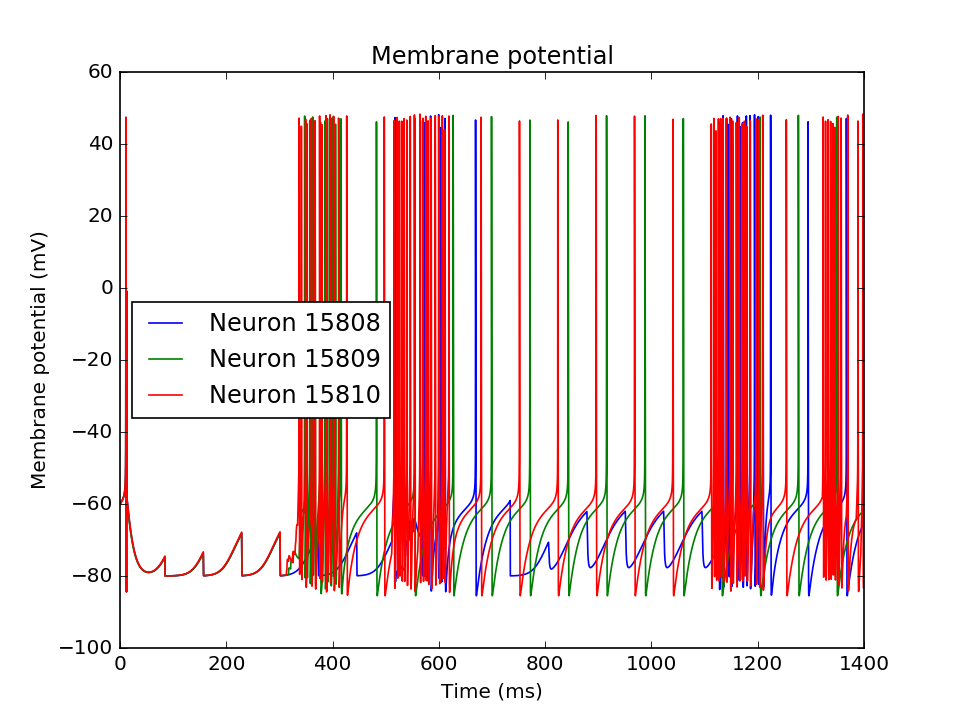
\includegraphics[width=0.5\linewidth]{volt_vta[da0]}
	\caption{Изменение потенциала мембраны некоторых нейронов в вентральной области покрышки.}
	\label{fig:volt_vta}
\end{figure}

\begin{figure}
	\centering
	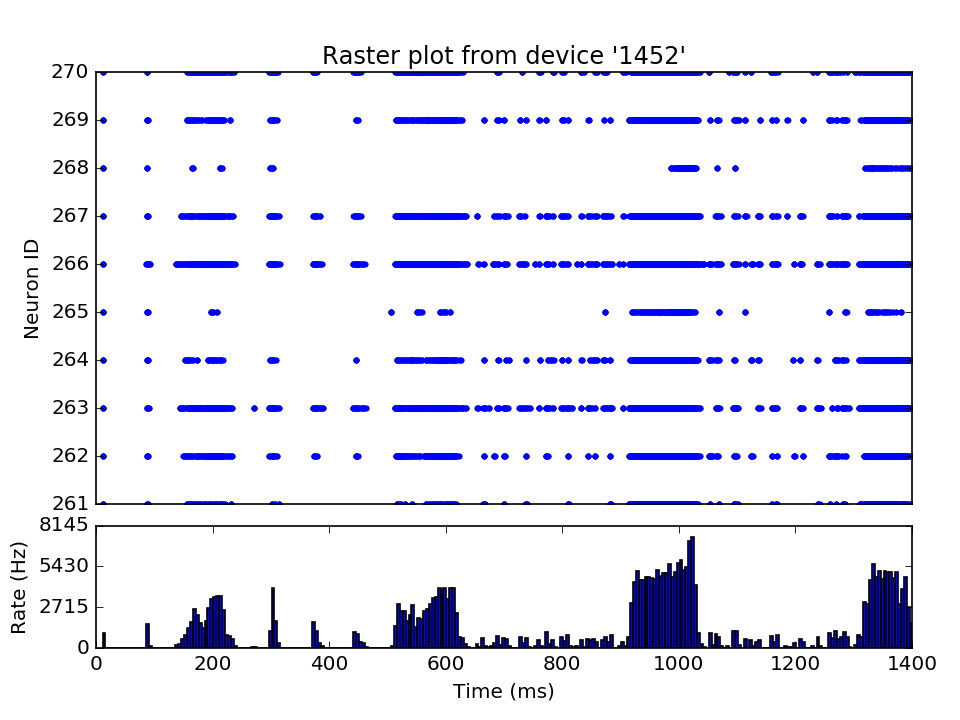
\includegraphics[width=0.5\linewidth]{spikes_striatum[tan]}
	\caption{Спайковая активность в стриатуме.}
	\label{fig:spikes_striatum}
\end{figure}

\begin{figure}
	\centering
	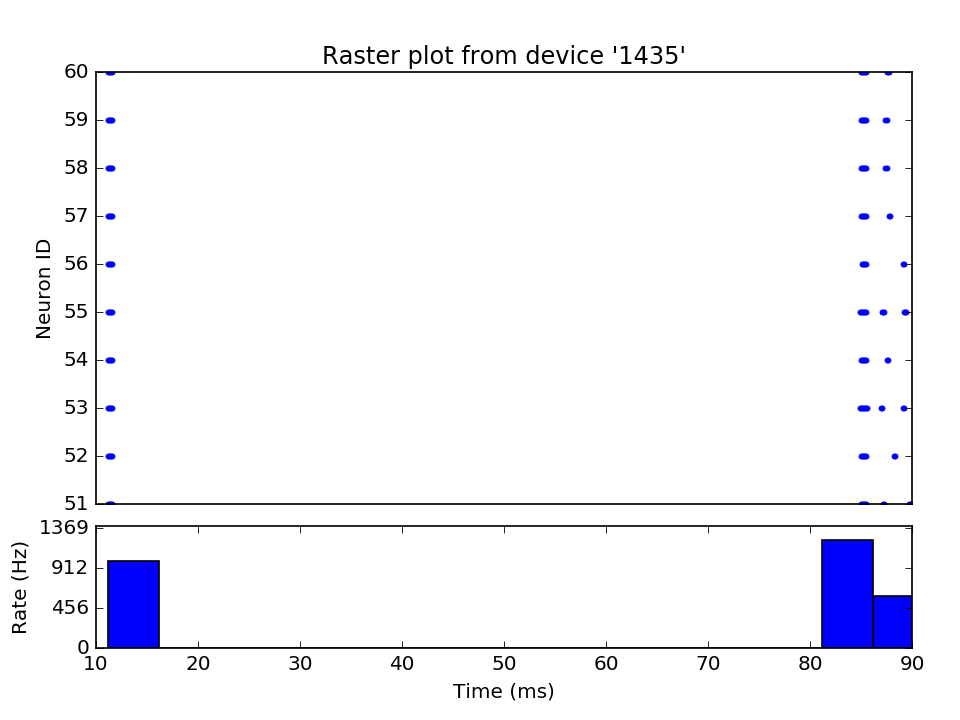
\includegraphics[width=0.5\linewidth]{spikes_thalamus}
	\caption{Спайковая активность в таламусе.}
	\label{fig:spikes_thalamus}
\end{figure}


\item Главные области, испытывающие проекции всех нейромодуляторов (моторная кора, сенсорная кора, префронтальная кора).

\begin{figure}
	\centering
	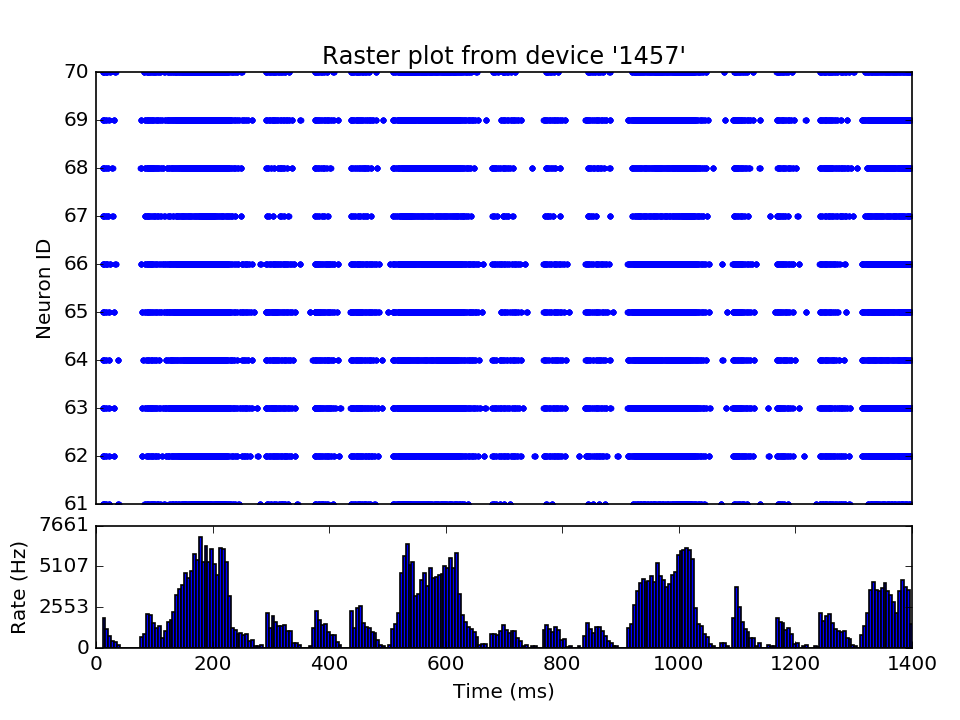
\includegraphics[width=0.5\linewidth]{spikes_motor[glu1]}
	\caption{Спайковая активность в моторной коре.}
	\label{fig:spikes_motor}
\end{figure}

\begin{figure}
	\centering
	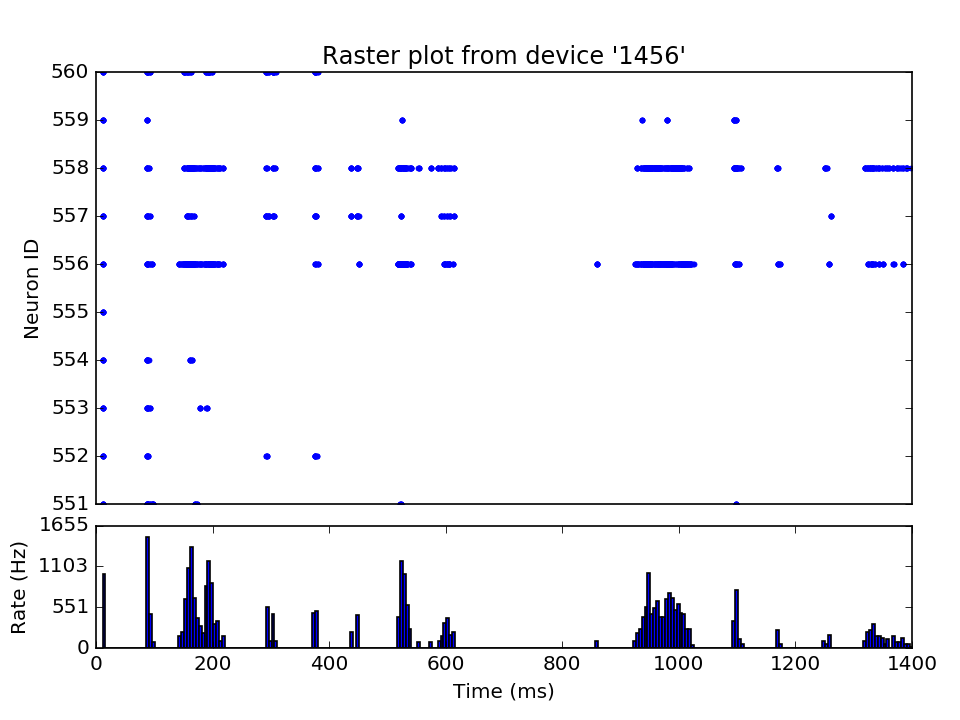
\includegraphics[width=0.5\linewidth]{spikes_motor[glu0]}
	\caption{Спайковая активность в сенсорной коре.}
	\label{fig:spikes_sensory}
\end{figure}


\begin{figure}
	\centering
	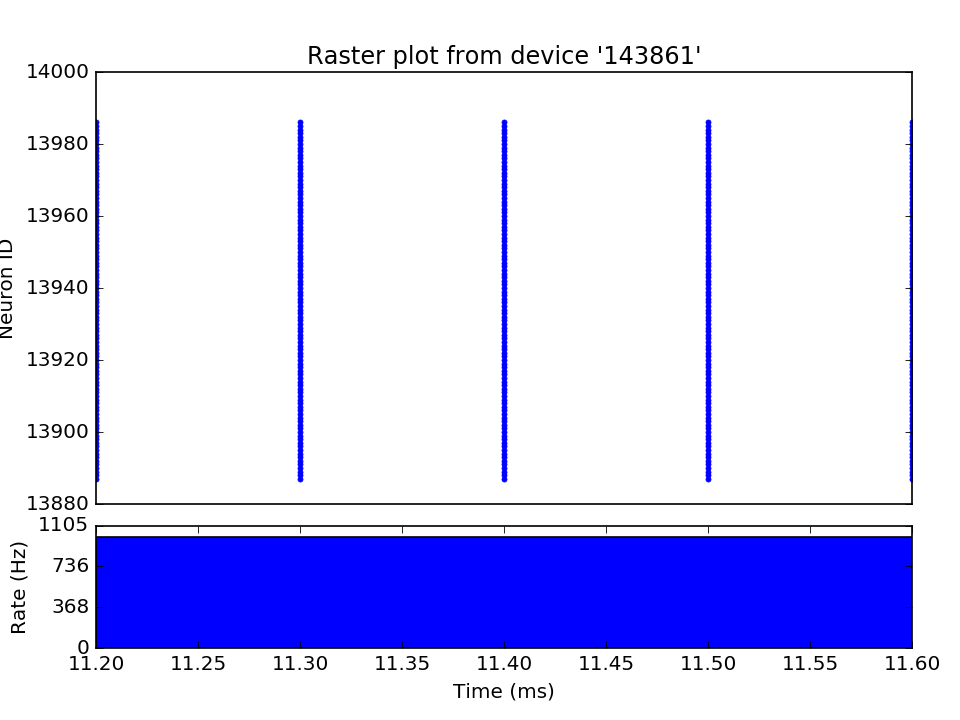
\includegraphics[width=0.5\linewidth]{spikes_prefrontal}
	\caption{Спайковая активность в префронтальной коре.}
	\label{fig:spikes_prefrontal}
\end{figure}


\end{itemize}

